% *********************************************************************
% © 2010–2026 Jeremy Sylvestre
%
% Permission is granted to copy, distribute and/or modify this document
% under the terms of the GNU Free Documentation License, Version 1.3 or
% any later version published by the Free Software Foundation; with no
% Invariant Sections, no Front-Cover Texts, and no Back-Cover Texts. A
% copy of the license is included in the appendix entitled “GNU Free
% Documentation License” that appears in the output document of this
% PreTeXt source code. All trademarks™ are the registered® marks of
% their respective owners.
%
% *********************************************************************

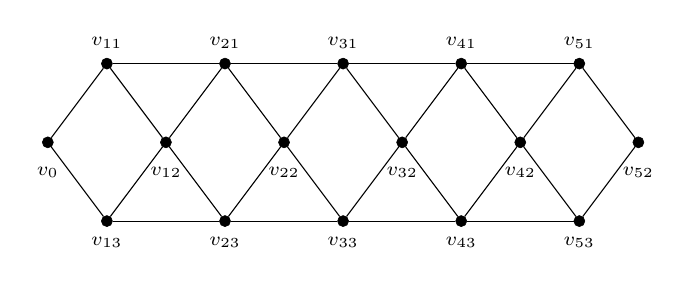
\begin{tikzpicture}[
	xscale=1.5,
	vertex/.style={ circle, draw, very thin, fill, inner sep=0pt, minimum size=4pt },
	vertexg/.style={ black!40!white, circle, draw, very thin, fill, inner sep=0pt, minimum size=4pt },
	vertexo/.style={ circle, draw, very thin, inner sep=0pt, minimum size=4pt }
]

\node at (0.5,0) (v0) [vertex,label={[yshift=-0.65cm]$\scriptstyle v_0$}] {};
\foreach \p in {1,2,3,4,5} {
	\begin{scope}[xshift=\p cm]
		\node at (0,1) (v\p1) [vertex,label=above:$\scriptstyle v_{\p1}$] {};
		\node at (0.5,0) (v\p2) [vertex,label={[yshift=-0.65cm]$\scriptstyle v_{\p2}$}] {};
		\node at (0,-1) (v\p3) [vertex,label=below:$\scriptstyle v_{\p3}$] {};
		\draw (v\p1) to (v\p2) to (v\p3);
	\end{scope}
}
\foreach \p in {1,3} \draw (v1\p) to (v2\p) to (v3\p) to (v4\p) to (v5\p);
\draw (v11) to (v0) to (v13);
\draw (v21) to (v12) to (v23);
\draw (v31) to (v22) to (v33);
\draw (v41) to (v32) to (v43);
\draw (v51) to (v42) to (v53);

\end{tikzpicture}
